%%%%%%%%%%%%%%%%%%%%%%%%%%%%%%%%%%%%%%%%%%%%%%%%%%%%%%%%%%%%%%%%%%%
%%%%%%%%%%%%%%%%%%%%%%%%%%%%%%%%%%%%%%%%%%%%%%%%%%%%%%%%%%%%%%%%%%%
\section{Introdução} % Sections can be created in order to organize your presentation into discrete blocks, all sections and subsections are automatically printed in the table of contents as an overview of the talk

%%%%%%%%%%%%%%%%%%%%%%%%%%%%%%%%%%%%%%%%%%%%%%%%%%%%%%%%%%%%%%%%%%%
\subsection{Agricultura de precisão}

\begin{frame}
\frametitle{Agricultura de precisão}
\begin{columns}

	\column{0.7\linewidth}
	\begin{figure}[]
	 \centering
	 \captionsetup{width=0.9\textwidth,font=footnotesize,textfont=bf}
	 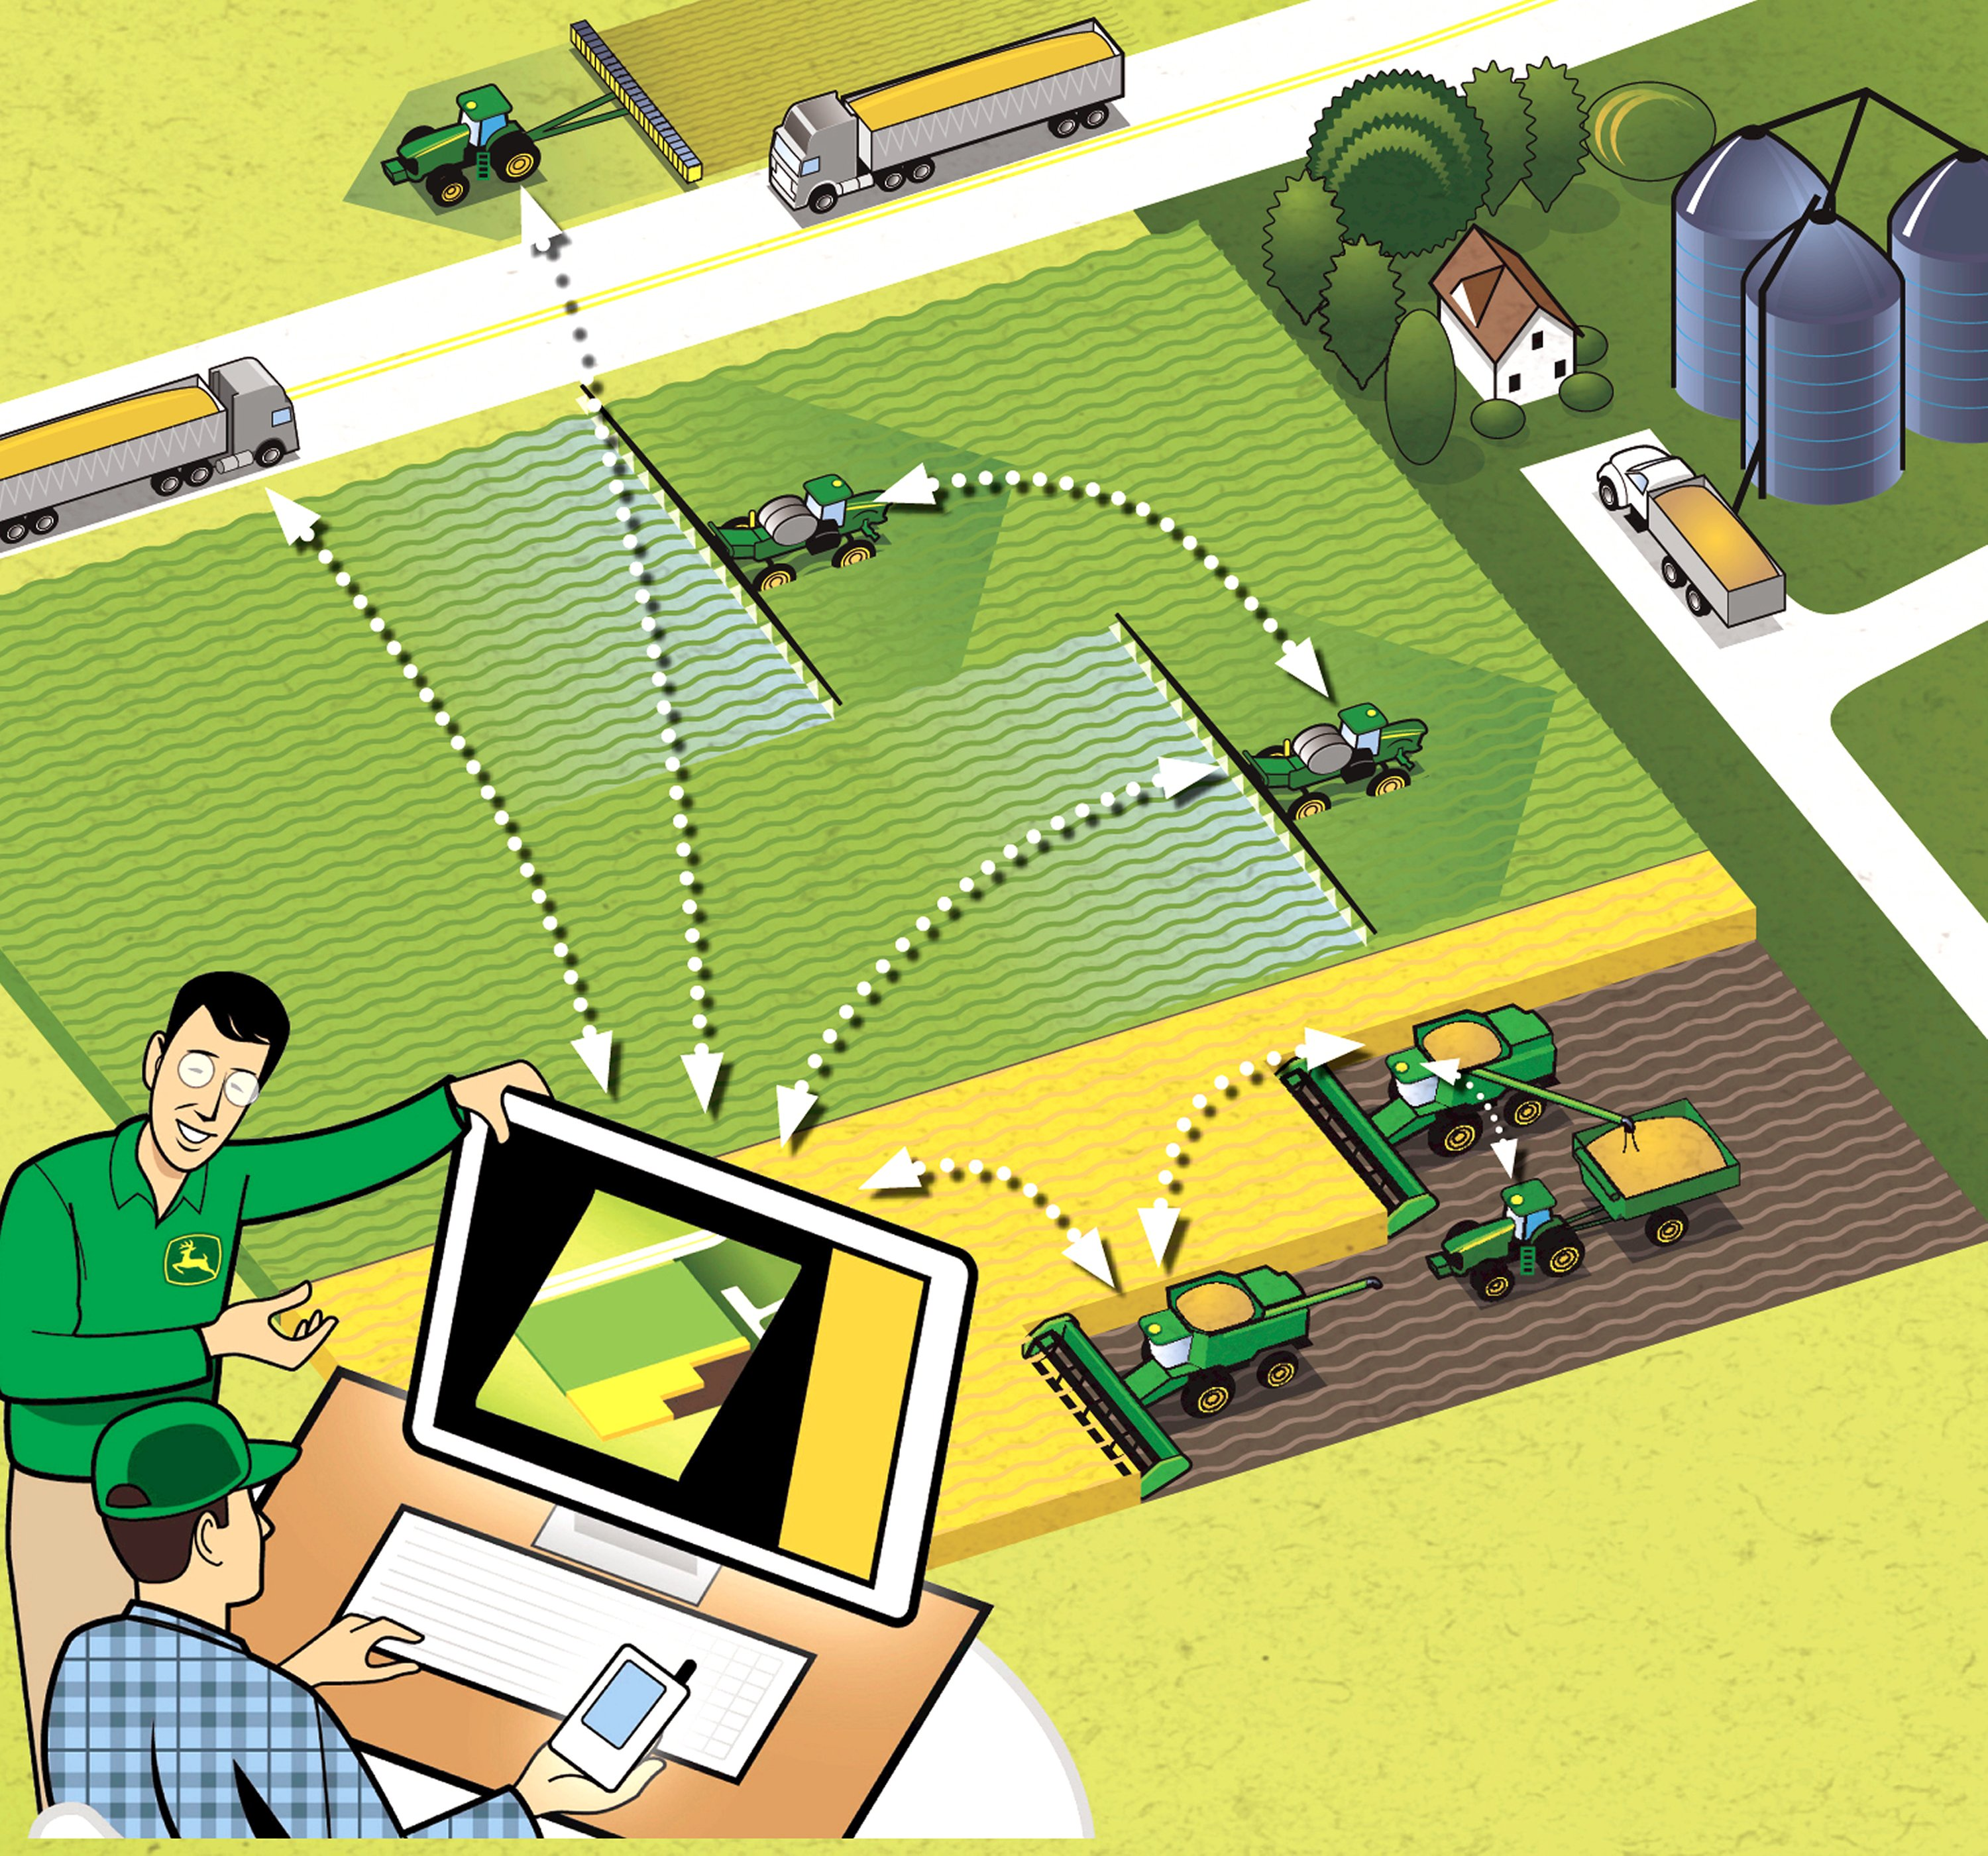
\includegraphics[width=0.9\textwidth,keepaspectratio]{Figuras/precisao.jpg}
	 \caption{Agricultura de precisão}
	\end{figure}
	
	\column{0.4\linewidth}
	\begin{itemize}
	\item \textbf{Conceito:}
	\item \textit{Sistema de Gerenciamento agrícola baseado na variação espacial e temporal da unidade produtiva e que visa aumento de retorno econômico, sustentabilidade e minimização do efeito no ambiente}
	\end{itemize}

\end{columns}
\end{frame}

\begin{frame}
\frametitle{Agricultura de precisão}
\begin{columns}

	\column{0.7\linewidth}
	\begin{figure}[]
	 \centering
	 \captionsetup{width=0.9\textwidth,font=footnotesize,textfont=bf}
	 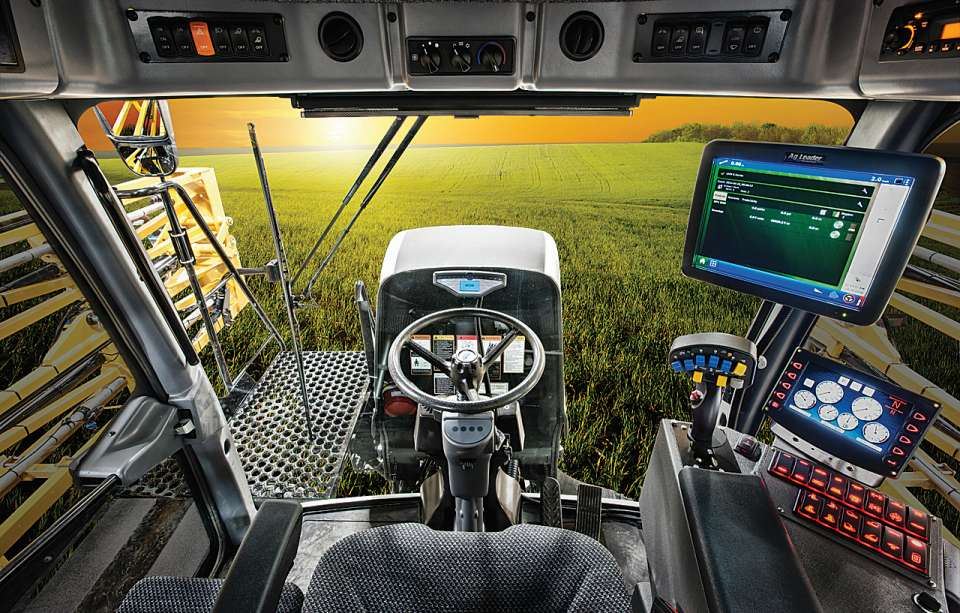
\includegraphics[width=0.9\textwidth,keepaspectratio]{Figuras/auto.jpg}
	 \caption{Automação agrícola}
	\end{figure}
	
	\column{0.4\linewidth}
	\begin{itemize}
	\item Sensores
	\item GPS
	\item Sistemas automatizados
	\end{itemize}

\end{columns}

\end{frame}

%%%%%%%%%%%%%%%%%%%%%%%%%%%%%%%%%%%%%%%%%%%%%%%%%%%%%%%%%%%%%%%%%%%
\subsection{GPS}

\begin{frame}
\frametitle{GPS}
\begin{columns}

	\column{0.7\linewidth}
	\begin{figure}[]
	 \centering
	 \captionsetup{width=0.9\textwidth,font=footnotesize,textfont=bf}
	 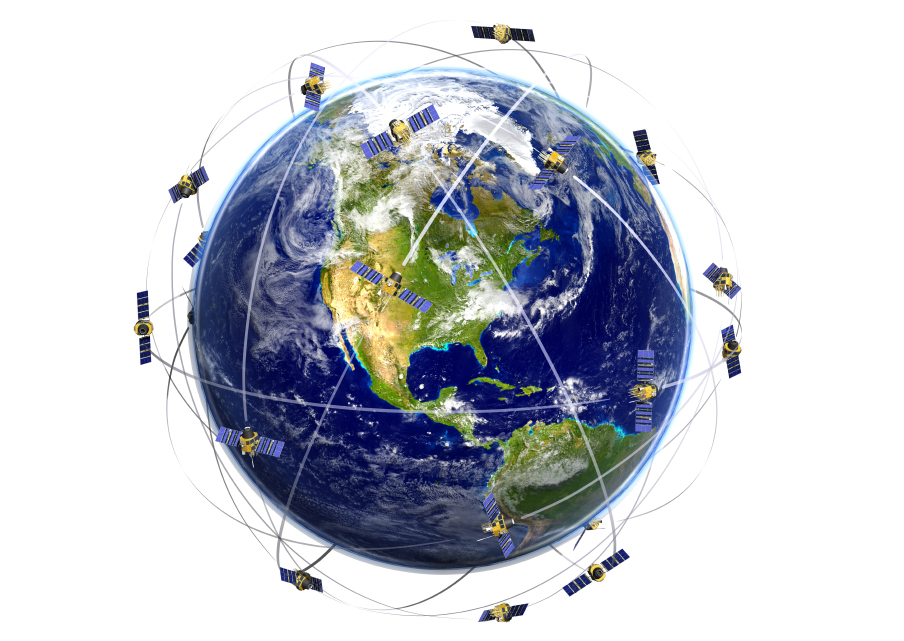
\includegraphics[width=0.9\textwidth,keepaspectratio]{Figuras/gps.jpg}
	 \caption{Sistema GPS}
	\end{figure}
	
	\column{0.4\linewidth}
	\begin{itemize}
	\item \textit{Global Position System} (Sistema de Posicionamento Global)
	\pause
	\item Padrão de comunicação NMEA (\textit{National Marine Electronics Association} ou Associação Nacional de Eletrônica Marinha)
	\item Sentenças começam com um '\$'.
	\end{itemize}

\end{columns}
\end{frame}

%%%%%%%%%%%%%%%%%%%%%%%%%%%%%%%%%%%%%%%%%%%%%%%%%%%%%%%%%%%%%%%%%%%
%\subsection{Microcontrolador}
%
%\begin{frame}
%\frametitle{Microcontrolador}
%\begin{columns}
%
%	\column{0.7\linewidth}
%	\begin{figure}[]
%	 \centering
%	 \captionsetup{width=0.9\textwidth,font=footnotesize,textfont=bf}
%	 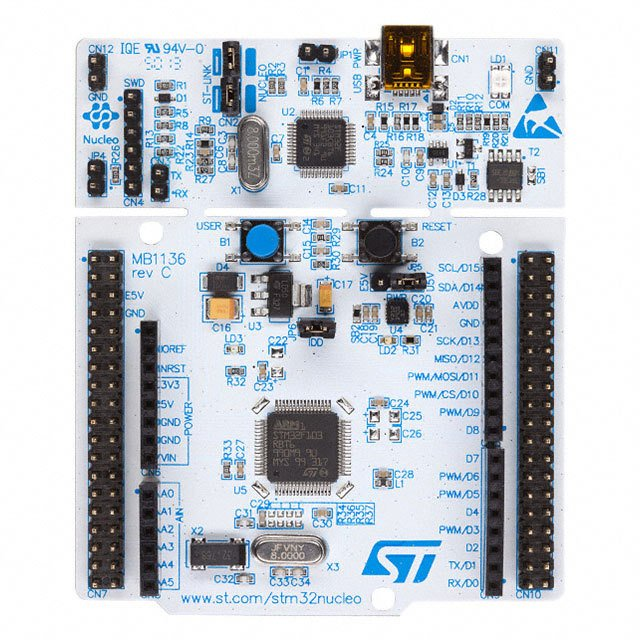
\includegraphics[width=0.9\textwidth,keepaspectratio]{Figuras/nucleo.jpg}
%	 \caption{Nucleo-STM32F030R8}
%	\end{figure}
%	
%	\column{0.4\linewidth}
%	\begin{itemize}
%	\item Computador embarcado
%	\pause
%	\item 
%	\item Sentenças começam com um '\$'.
%	\end{itemize}
%
%\end{columns}
%\end{frame}





%%%%%%%%%%%%%%%%%%%%%%%%%%%%%%%%%%%%%%%%%%%%%%%%%%%%%%%%%%%%%%%%%%%%%%%%%%%%%%%%%
%%%%%%%%%%%%%%%%%%%%%%%%%%%%%%%%%%%%%%%%%%%%%%%%%%%%%%%%%%%%%%%%%%%%%%%%%%%%%%%%

\section{Plano de estágio}

\subsection{A Empresa}

\begin{frame}%[noframenumbering]
\frametitle{A empresa}
\begin{columns}

	\column{0.7\linewidth}
	\begin{figure}[]
	 \centering
	 \captionsetup{width=\textwidth,font=footnotesize,textfont=bf}
	 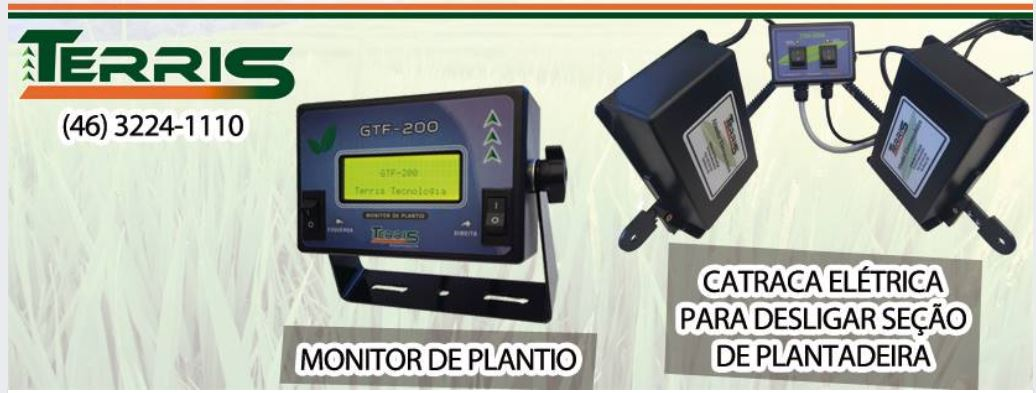
\includegraphics[width=\textwidth,keepaspectratio]{Figuras/Terris.jpg}
	 \caption{Logo da Terris}
	\end{figure}
	
	\column{0.4\linewidth}
	\begin{itemize}
	\item Terris automação agrícola
	\pause
	\item Empresa encubada
	\pause
	\item Produtos desenvolvidos e comercializados
	\end{itemize}

\end{columns}
\end{frame}

%%%%%%%%%%%%%%%%%%%%%%%%%%%%%%%%%%%%%%%%%%%%%%%%%%%%%%%%%%%%%%%%%%%%%%
\subsection{O Estágio}

\begin{frame}
\frametitle{O Estágio}

\begin{itemize}
	\item \textbf{Área de atuação}: Pesquisa e desenvolvimento
	\pause
	\item \textbf{Tipo de estágio}: Estudo dirigido
	\pause
	\item \textbf{Setor da empresa}: Automação agrícola
	\pause	
	\item \textbf{Orientador(a)}: Professora Dra. Beatriz Terezinha Borsoi
	\pause
	\item \textbf{Contatos na empresa}: \\Sidney Gaspari\\ Josimar Tumeleiro
\end{itemize}
\end{frame}

%%%%%%%%%%%%%%%%%%%%%%%%%%%%%%%%%%%%%%%%%%%%%%%%%%%%%%%%%%%%%%%%%%%%%%%%%%%%%
%\subsection{Atividade desenvolvida}
\begin{frame}
\frametitle{O Estágio}

\begin{block}{Atividade desenvolvida}
\begin{itemize}
\item Estudo comparativo entre os módulos \textit{Global Position System} (GPS), ou Sistema de Posicionamento Global, verificando a sua aplicabilidade na agricultura de precisão.
\pause 
\item Programação dos sensores utilizando o microcontrolador STM32F030R8, da STMicroelectronics\textregistered, visando a aplicação dos módulos estudados em um produto comercial desenvolvida pela empresa Terris\textregistered, que trabalha com o desenvolvimento de tecnologias agrícolas.
\end{itemize}
\end{block}

\end{frame}


%%%%%%%%%%%%%%%%%%%%%%% EOF %%%%%%%%%%%%%%%%%%%%%%%%%%%%